% !TeX root = ../paper.tex

\section{Introduction}

This chapter is based on material from the following publications:

\begin{mdframed}
\begin{center} 
    \bibentry{van2023snekhorn} 
\end{center}
\end{mdframed}

\begin{mdframed}
    \begin{center} 
        \bibentry{van2023optimal} 
    \end{center}
\end{mdframed}

It focuses on addressing \Cref{prob:adaptive_ds}, which aims to reconcile entropic affinities (\Cref{sec:background_dr}) with symmetric doubly stochastic ones (\Cref{sec:doubly_sto}). In other words, it involves finding the appropriate method for symmetrizing entropic affinities.
The Euclidean projection used in t-SNE, $\overline{\Pb^{\mathrm{e}}} = \frac{1}{2} \left( \Pb^{\mathrm{e}} + \Pb^{\mathrm{e} \top} \right)$, is inadequate because it \emph{fails to preserve the structure of the entropic affinities}.
In particular, $\overline{\Pb^{\mathrm{e}}}$ is not stochastic in
general and $\operatorname{H}(\overline{\Pb_{i:}^{\mathrm{e}}}) \neq (\log{\xi} + 1)$ thus the entropy associated with each point is no longer controlled after symmetrization (see the bottom left plot of \Cref{fig:coil}). This is
arguably one of the main drawbacks of the approach. By contrast, the
$\Pb^{\mathrm{se}}$ affinity that will be introduced in \Cref{sec:sym_entropic_affinity} can
accurately set the entropy in each point to the desired value $\log \xi + 1$.  As shown in \Cref{fig:coil} this leads to more faithful embeddings with higher silhouette scores when combined with the SNEkhorn algorithm (\Cref{sec:DR_with_OT}).

\begin{figure}
    \centering
    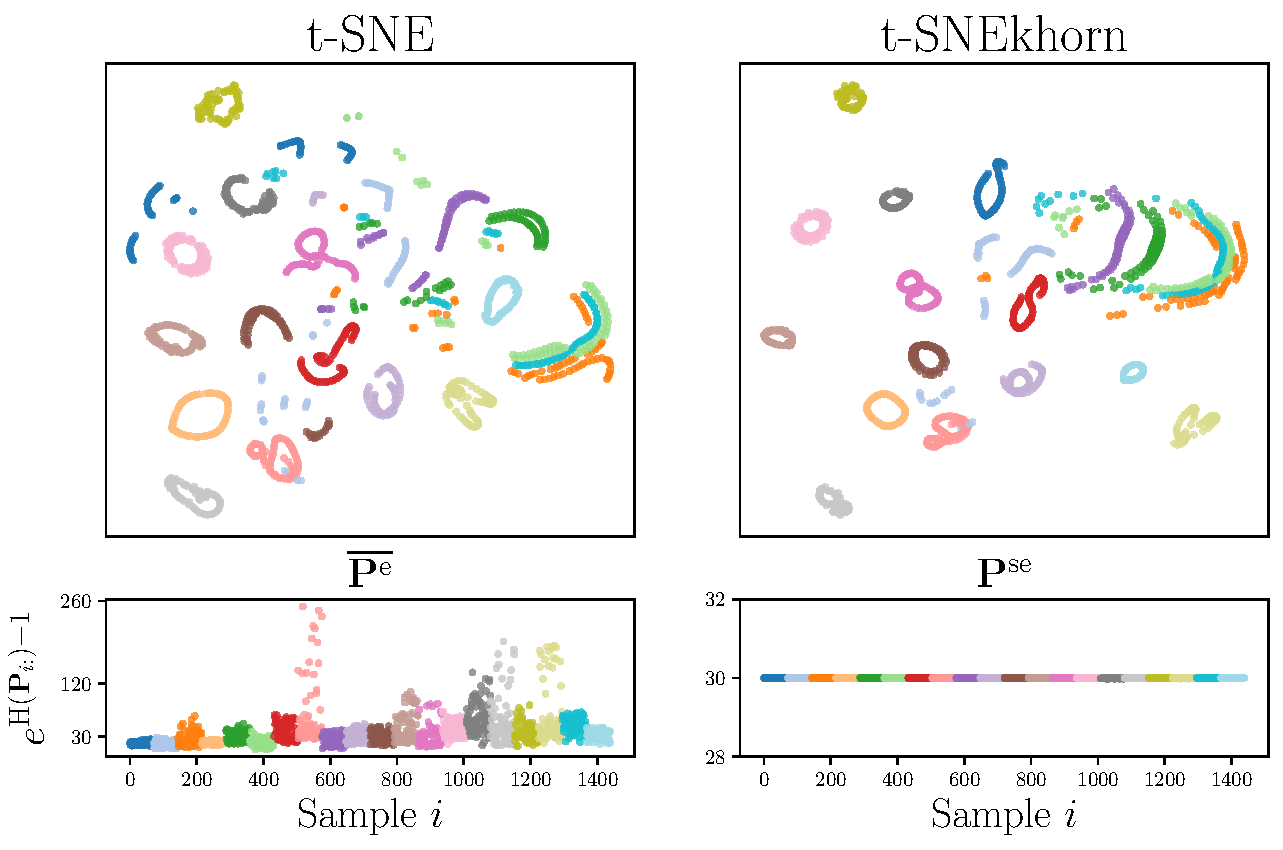
\includegraphics[width=0.6\linewidth]{figures/SNEkhorn/fig_coil.pdf}
    \caption{Top: COIL \cite{nene1996columbia} embeddings with silhouette scores produced by Symmetric-SNE and SNEkhorn (our method introduced in  \Cref{sec:DR_with_OT}) for $\xi=30$. Bottom: $e^{\operatorname{H}(\Pb_{i:})-1}$ (\emph{perplexity}) for each point $i$.}
    \label{fig:coil}
\end{figure}

\paragraph{Outline.} In this work, we study the missing
link between EAs, which are easy to tune and adaptable to data with heterogeneous density, and doubly stochastic affinities which have interesting properties in practical applications as seen in \Cref{sec:doubly_sto}. 
%To this end, we tackle two major challenges.
%Extending entropic affinities from stochastic to
%doubly stochastic seems promising given all the aforementioned benefits. 
%However, two main challenges appear. 
% First, the current formulation of entropic affinities is specifically tailored for directed stochastic affinities. Secondly, as pointed out in \citep{lu2019doubly}, when one
% runs t-SNE with a doubly stochastic affinity, low dimensional
% coordinates tend to concentrate on spheres thus making embedding onto a 2D
% surface (typical use case of DR) of limited use \titouan{a reformuler ces deux phrases: la deuxieme est effectivement un challenge mais je ne comprends pas en quoi ce qu'on fait le résoud, et le premier c'est pas vraiment un challenge, c'est juste que ça n'existe pas}\nc{agree with that}.  
Our main contributions are as follows. We uncover the convex
optimization problem that underpins classical entropic affinities, exhibiting
novel links with entropy-regularized Optimal Transport (OT) (\Cref{sec:entropic_affinity_semi_relaxed}). We then propose in \Cref{subsec:sea} a principled symmetrization of entropic
affinities. The latter enables controlling the entropy in each point, unlike
t-SNE's post-processing symmetrization, and producing a genuinely doubly stochastic affinity. We show how to
compute this new affinity efficiently using a dual ascent algorithm.
In \Cref{sec:DR_with_OT}, we introduce SNEkhorn: a DR algorithm that couples this new symmetric entropic affinity with a doubly stochastic kernel in the low-dimensional embedding space, without sphere concentration issue \cite{lu2019doubly}. We showcase the benefits of symmetric entropic affinities on a variety of applications in Section \ref{sec:DR_experiments} including spectral clustering and DR experiments on datasets ranging from images to genomics data. In \Cref{sec:OTARI}, we build upon these findings to introduce an adaptive version of regularized optimal transport.
